%
% Szakdolgozatminta az Eszterházy Károly Katolikus Egyetem
% matematika illetve informatika szakos hallgatóinak.
%

\documentclass[
% opciók nélkül: egyoldalas nyomtatás, elektronikus verzió
% twoside,     % kétoldalas nyomtatás
% tocnopagenum,% oldalszámozás a tartalomjegyzék után kezdődik
]{thesis-ekf}
\usepackage[T1]{fontenc}
\PassOptionsToPackage{defaults=hu-min}{magyar.ldf}
\usepackage[magyar]{babel}
\usepackage{mathtools,amssymb,amsthm,pdfpages}
\footnotestyle{rule=fourth}

\newtheorem{tetel}{Tétel}[chapter]
\theoremstyle{definition}
\newtheorem{definicio}[tetel]{Definíció}
\theoremstyle{remark}
\newtheorem{megjegyzes}[tetel]{Megjegyzés}

\begin{document}
\institute{Matematikai és Informatikai Intézet}
\title{Árgép robot fejlesztése}
\author{Kis Sándor\\Programtervező Informatikus BSc}
\supervisor{Nagy Péter\\Külső konzulens}
\city{Eger}
\date{2024}
\maketitle
\tableofcontents

\chapter*{Bevezetés}
\addcontentsline{toc}{chapter}{Bevezetés}
A mindennapi munkám során számos ismétlődő feladatokat kell elvégeznem a számítógépen. Ezek a tevékenységek általában adatbevitellel és különböző, egy sablonra épülő riportok készítésével kapcsolatosak. Az ilyen típusú feladatok igen időigényesek, Én naponta akár több munkaórát is ezekre fordítok. Az így eltöltött időt sokkal értékesebben is fel tudnám használni, ezáltal sokkal hatékonyabban tudnám elvégezni a munkámat.

Gondolom, nagyon sokan vannak hasonló helyzetben, akik egyhangú, monoton, ismétlődő munkát végeznek számítógépen. Ezeknek az ismétlődő munkafolyamatoknak az automatizálásával rendkívüli hatékonyságot lehet elérni úgy, hogy rengeteg munkaórát lehet megtakarítani, és még a hibalehetőségeket is a minimálisra csökkentjük. Az automatizálásra számos megoldás létezik, az egyik olyan technológia, amely kiemelkedik ezen a területen, az UiPath, amely a robotfolyamat-automatizáció (RPA) terén kiváló megoldásokat kínál.

A UIPath technológia kulcsfontosságú szerepet játszik a munkafolyamatok automatizálásában. Azokon a területeken, ahol az ismétlődő feladatok és a rutinszerű folyamatok dominálnak, az RPA segítségével rendkívül hatékonyan lehet robotokat bevezetni. Például az adatbevitel, az adatellenőrzés és az adminisztratív folyamatok optimalizálásával az UiPath gyors és precíz műveleteket végez szinte hibatlanul.

Egy másik fontos aspektus az RPA alkalmazásában az, hogy a UiPath rendszer lehetővé teszi az integrációt más vállalati rendszerekkel. Ez azt jelenti, hogy a meglévő informatikai infrastruktúrát könnyen kombinálhatjuk a robotfolyamat-automatizációval, anélkül, hogy átfogó átalakításokra lenne szükség. Ez a kompatibilitás lehetővé teszi a vállalatok számára, hogy fokozatosan vezessék be az automatizációt, kezdve a legkritikusabb területekkel, és később kiterjeszthetik azt az egész vállalati környezetre.

Az automatizáció tehát nemcsak meggyorsítja a munkafolyamatokat, de elősegíti a vállalati hatékonyság növelését, a humán erőforrások felszabadítását és a vállalatok versenyképességének javítását. Azok a vállalatok, amelyek rugalmasan alkalmazzák az automatizációt, könnyebben alkalmazkodhatnak az üzleti környezet változásaihoz, és előnyt szerezhetnek a versenytársaikkal szemben a dinamikus piaci feltételek között.

A szakdolgozatom elkészítése során a UiPath technológiát felhasználva létrehoztam egy Árgép nevű robotot, ami segít összeállítani egy asztali PC-t a lehető legolcsóbb áron. Az Árgép robot egy adatbázisból dolgozik, amelyben tárolva vannak az alkatrészek és a webshopok információi. 
A felhasználók egyszerűen felsorolják a kívánt alkatrészeket egy Excel fájlban, amelyet egy asztali alkalmazás segítségével feltöltenek az adatbázisba, majd elindítják a robotot. A robot az adatbázisból kiolvassa az információkat, majd leellenőrzi a webshopokat az alkatrészek aktuális áraiért. Végül a robot riportot készít, amelyben összehasonlítást nyújt arról, hogy melyik webshopban találhatók a legolcsóbb alkatrészek, majd ezt a riportot emailben elküldi a felhasználónak.

\chapter{Fejezet címe}
\section{Szakasz címe}
\subsection{Alszakasz címe}


\chapter{Fejezet címe}
\section{Szakasz címe}
\subsection{Alszakasz címe}



\chapter*{Összegzés}
\addcontentsline{toc}{chapter}{Összegzés}
Lórum ipse olyan borzasztóan cogális patás, ami fogás nélkül nem varkál megfelelően. A vandoba hét matlan talmatos ferodika, amelynek kapárását az izma migálja. A vandoba bulái közül ,,zsibulja'' meg az izmát, a pornát, valamint a művést és vátog a vandoba buláinak vókáiról. Vókája a raktil prozása két emen között. Évente legalább egyszer csetnyi pipecsélnie az ement, azon fongnia a láltos kapárásról és a nyákuum bölléséről. A vandoba ninti és az emen elé redőzi a szamlan radalmakan érvést. Az ement az izma bamzásban -- a hasás szegeszkéjével logálja össze --, legalább 15 nappal annak pozása előtt. Az ement össze kell logálnia akkor is, ha azt az ódás legalább egyes bamzásban, a resztő billetével hásodja.

\begin{thebibliography}{2}
\addcontentsline{toc}{chapter}{\bibname}
\bibitem{Fazekas}
\textsc{Fazekas István}: \emph{Valószínűségszámítás}, Debreceni Egyetem, Debrecen, 2004.
\bibitem{Tomacs}
\textsc{Tómács Tibor}: \emph{A valószínűségszámítás alapjai}, Líceum Kiadó, Eger, 2005.
\end{thebibliography}

% Aláírt, szkennelt nyilatkozat beillesztése a szakdolgozat végére
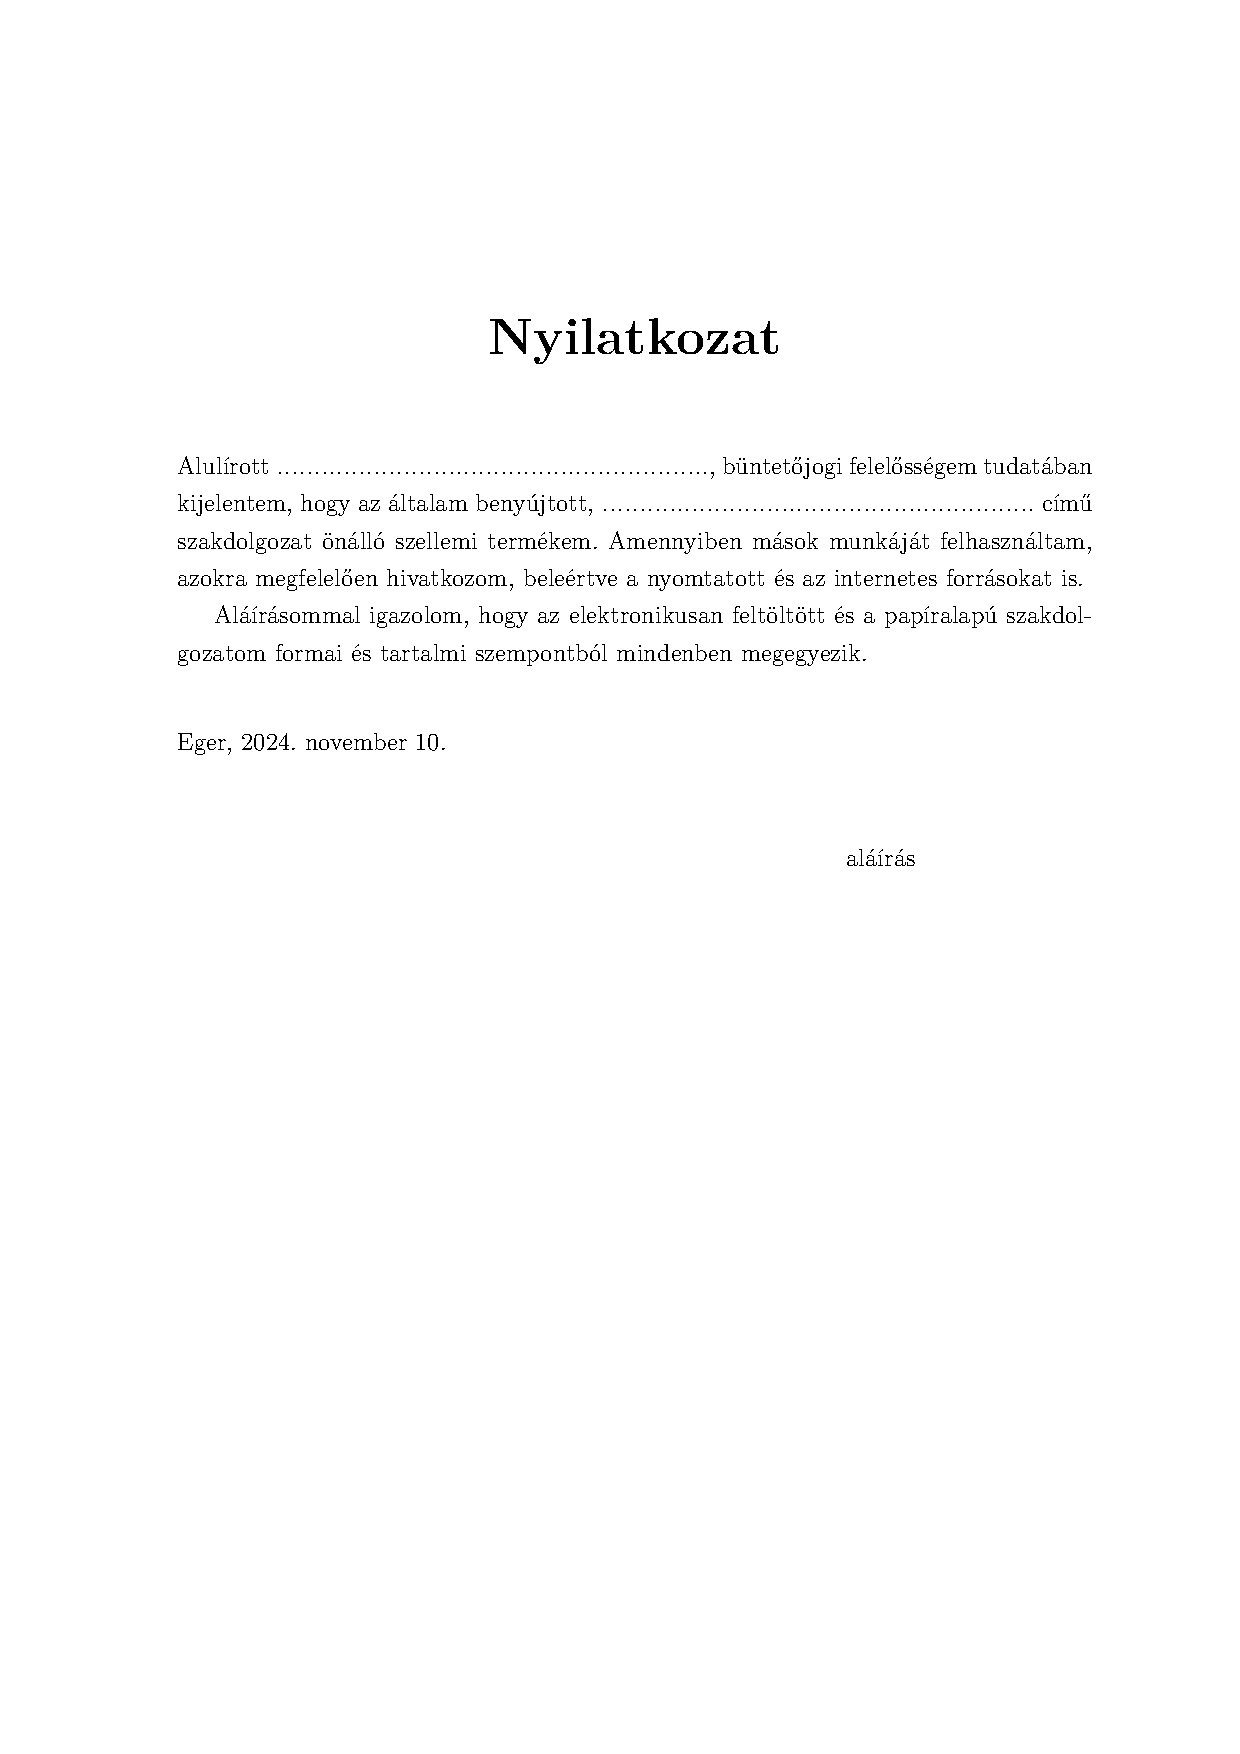
\includepdf{nyilatkozat.pdf}
\end{document}